%%%%%%%%%%%%%%%%%%%%%%%%%%%%%%%%%%%%%%%%%%%%%%%%%%%%%%%%%%%%%%%%%%%%%%%%%%%%%%%
%% StuPro A, Produktlinien (Kobold)
%% Team Werkbold
%% Anforderungsdokument
%% $Id: anforderungsdokument.tex,v 1.9 2004/02/24 15:41:15 garbeam Exp $
%%%%%%%%%%%%%%%%%%%%%%%%%%%%%%%%%%%%%%%%%%%%%%%%%%%%%%%%%%%%%%%%%%%%%%%%%%%%%%%
\documentclass[a4paper,titlepage,12pt,ngerman]{scrbook}
\usepackage{../common/header}
\usepackage{supertabular}

\RCSdef $Revision: 1.9 $
\RCSdef $Date: 2004/02/24 15:41:15 $

%\newcommand\version{Version \today \xspace}
\newcommand\version{Version 1.0\xspace}

\title {\huge \product\\[0.5cm]\large Projektplan \\[0.5cm] \version
  \\[1cm] \Large \company}

\begin{document}

%%%%%%%%%%%%%%%%%%%%%%%%%%%%%%%%%%%%%%%%%%%%%%%%%%%%%%%%%%%%%%%%%%%%%%%%%%%%%%%
%% Deckblatt

\begin{titlepage}
\renewcommand{\thefootnote}{\fnsymbol{footnote}}
{\Huge
\raggedright
\textbf{\bf Kobold} \\
\huge Produktlinien Management System
\rule{\textwidth}{0.75pt}
\par
}
\begin{flushleft}
\normalsize
\version
\end{flushleft}

\vspace*{3cm}
\begin{center}

\includegraphics[width=15cm]{../common/logo-color.png}
\end{center}
\vfill

{\parindent=0cm
\Huge Anforderungsdokument
}


\setcounter{footnote}{0}
\end{titlepage}

%%%%%%%%%%%%%%%%%%%%%%%%%%%%%%%%%%%%%%%%%%%%%%%%%%%%%%%%%%%%%%%%%%%%%%%%%%%%%%%
%% Versionsgeschichte

\section*{Versionsgeschichte}

\begin{itemize}

\item Version 1.0  ($Id: anforderungsdokument.tex,v 1.9 2004/02/24 15:41:15 garbeam Exp $)


\end{itemize}

%%%%%%%%%%%%%%%%%%%%%%%%%%%%%%%%%%%%%%%%%%%%%%%%%%%%%%%%%%%%%%%%%%%%%%%%%%%%%%%
%% Inhaltsverzeichnis

\tableofcontents
%%%%%%%%%%%%%%%%%%%%%%%%%%%%%%%%%%%%%%%%%%%%%%%%%%%%%%%%%%%%%%%%%%%%%%%%%%%%%%%%%%% funktionale Anforderungen
%%%%%%%%%%%%%%%%%%%%%%%%%%%%%%%%%%%%%%%%%%%%%%%%%%%%%%%%%%%%%%%%%%%%%%%%%%%%%%%
%% StuPro A, Produktlinien (Kobold)
%% Team Werkbold
%% Angebot
%% $Id: produktanatomie.tex,v 1.1 2004/01/28 18:10:49 garbeam Exp $
%%%%%%%%%%%%%%%%%%%%%%%%%%%%%%%%%%%%%%%%%%%%%%%%%%%%%%%%%%%%%%%%%%%%%%%%%%%%%%%


\chapter{Architekturentscheidungen}

Erg�nzend zum Angebot werden in diesem Dokument die Architekturentscheidungen
n�her erl�utert und ein erweiterter �berblick zum GUI-Prototypen
zusammengefasst, der in der Angebotspr�sentation demonstriert wurde.
\par
\product wird in Form einer {\it J2SE}\footnote{Java 2 Standard Edition,
n�here Informationen unter: http://java.sun.com/j2se/}
 basierten Client-Server Architektur realisiert. Diese Entscheidung
beruht auf der systematischen Abw�gung von Vor- und Nachteilen zwischen
J2SE/Eclipse und GTK/Ada.\par Ada wird von den Werkbold-Entwicklern als
geeignete Entwicklungsumgebung f�r Systeme gesehen, die keine grafische
Benutzungsoberfl�che besitzen sowie f�r einen stand-alone Betrieb
ausgelegt sind, d.h. ohne komplexere Netzwerkanbindung (z.B. Compiler).
Die Anforderungsanalyse ergab hingegen, dass \product als plattformunabh�ngige
GUI-Anwendung mit Netzwerkanbindung realisiert werden soll.\par
Dies spricht in besonderem Ma�e f�r J2SE in Kombination mit der Eclipse
Plattform. Im Folgenden sind die Eigenschaften von J2SE/Eclipse und 
GTK/Ada aufgef�hrt, die zur Entscheidung f"ur die J2SE/Eclipse f"uhrten.\par
Vorteilhaft bewertete Eigenschaften sind mit einem (+) markiert, nachteilig
bewertete Eigenschaften sind mit einem (-) markiert.

\section{Eigenschaften von J2SE/Eclipse}
\begin{itemize}
\item Plattformunabh"angigkeit (+)
\item MVC-Konzept (+)
\item Hoher Verbreitagsgrad (+)
\item Guter Support (Community) (+)
\item Einfache Erweiterbarkeit (+)
\item VCM\footnote{Version Control Management} Unterst"utzung (+)
\item Grafiktoolkit SWT/JFace (+)
\item Gute Dokumentation (IBM) (+)
\item Netzwerktechnologie (+)
\end{itemize}

\section{Eigenschaften von GTK/Ada}
\begin{itemize}
\item Sauberes Sprachdesign (+)
\item Performante Visualisierung (+)
\item Kein natives Widget-Toolkit (-)
\item Abh"angigkeit von GTK (-)
\item "Ubersetzungsvorgang auf"andig (-)
\item Geringer Verbreitungsgrad von GUI-Applikationen (-)
\item Netzwerkanbindung komplex (-)
\item Keine VCM-Unterst"utzung (-)
\end{itemize}

\chapter{Der GUI-Prototyp}

Der Client wird als Plugin f�r die {\it Eclipse Platform}
\footnote{N�here Informationen: http://www.eclipse.org/}
realisiert, das die rollenbasierte Visualisierung und Verwaltung von
Produktlinienarchitekturen in Form von Graphen erm�glicht.\par
Dar�berhinaus dient der Client als Arbeitsumgebung f�r den Produktlinien- und
Produktingenieur sowie f�r den Entwickler. Alle im Produktlinien-Management
notwendigen Workflows k�nnen durch den Client angesto�en und entsprechend visualisiert
werden.

{\begin{center}
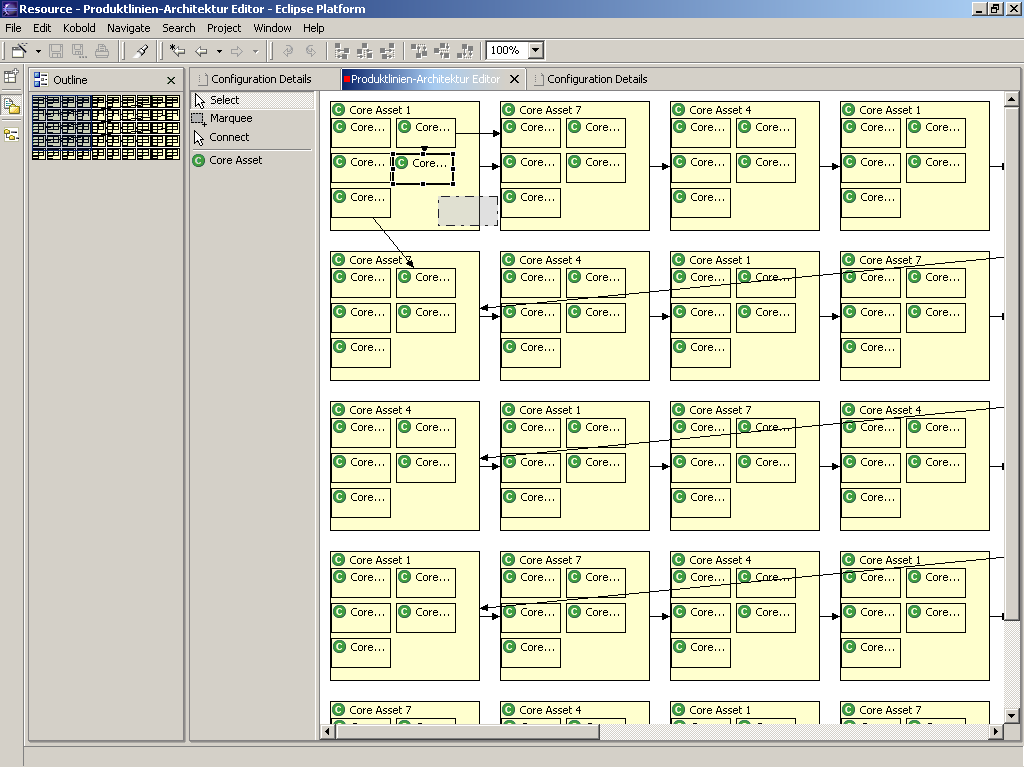
\includegraphics[width=15cm]{kobold-screen}\par
\small Abbildung der Eclipse-basierten Kobold GUI
\end{center}}

\section{Visualisierung}

Der Client visualisiert Produktlinien- und Produkt-Architekturen als Graphen
auf verschiedenen Abstraktionsebenen. Dabei stellt er alle Komponenten und deren
Abh�ngigkeiten (must-use und must-not-use) dar.

{\begin{center}
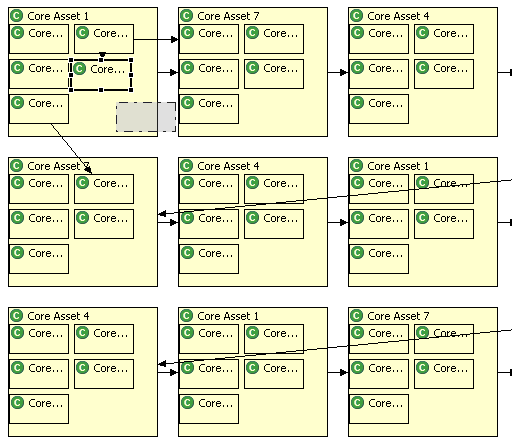
\includegraphics[width=10cm]{visual}\par
\small Ausschnitt aus einem Graphen
\end{center}}

\newpage
\section{Verwaltung}

Der Client verwaltet Produktlinien- und Produkt-Architekturen, d.h. er
erm�glicht die rollenbasierte Erstellung und Modifikation von
Architekturen.

{\begin{center}
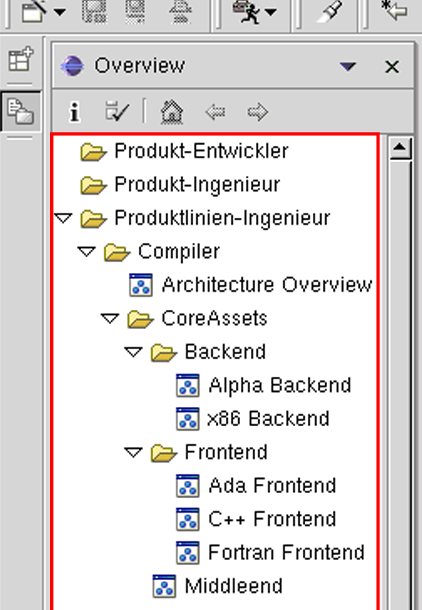
\includegraphics[width=5cm]{verwaltung}\par
\small Ausschnitt der Projektansicht
\end{center}}

\vspace*{2cm}
{\begin{center}
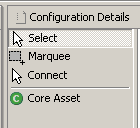
\includegraphics[width=3cm]{verwaltung2}\par
\small Ausschnitt der Manipulationsleiste
\end{center}}

%%% Local Variables: 
%%% TeX-master: "angebot"
%%% End: 
%%% vim:tw=79:


%%%%%%%%%%%%%%%%%%%%%%%%%%%%%%%%%%%%%%%%%%%%%%%%%%%%%%%%%%%%%%%%%%%%%%%%%%%%%%%
%% Anforderungen
%%%%%%%%%%%%%%%%%%%%%%%%%%%%%%%%%%%%%%%%%%%%%%%%%%%%%%%%%%%%%%%%%%%%%%%%%%%%%%%
%% StuPro A, Produktlinien (Kobold)
%% Team Werkbold
%% Anforderungsdokument
%%%%%%%%%%%%%%%%%%%%%%%%%%%%%%%%%%%%%%%%%%%%%%%%%%%%%%%%%%%%%%%%%%%%%%%%%%%%%%%

\chapter{Funktionale Anforderungen}
\section{Architekturanforderungen}
\begin{enumerate}
    \item Es kann mehrere Produktlinien geben
    \item Pro Programminstanz kann von einem Benutzer biliebiege Produktlinien bearbeitet werden
    \item Es muss m�glich sein, Skripte an jede VCM  Aktion. Werden mehrere Skripte bei einer Aktion ausgef�hrt. Die Reihenfolge ist durch Kobold vorgegeben. Skripte k�nnen an jede, Komponente, Variante, Produkt und Poduktlinie geh�ngt werden.
    \item Als VCM Aktionen muss es checkin, checkout, commit und update geben
    \item Es muss m�glich sein, die Architekturen verschiedener Produkte zu �berlappen und damit gleichzeitig anzuzeigen, um die Unterschiede und Gemeinsamkeiten dieser zu sehen. z.B.als Schnittgraph.
    \item Beim Anlegen und Bearbeiten von Architekturen soll das System �berpr�fen, ob diese korrekkonsistent sind. Wenn nicht, soll zwar eine Warnung gegeben werden, die Aktion soll aber trotzdem ausf�hrbar sein.
    \item F�r jede Komponente muss die M�glichkeit gegeben werden, Zust�ndigkeiten vergeben zu k�nnen, um bei Fragen oder Anregungen einen Ansprechpartner zu haben
    \item Auf der Produktlinienebene werden die explizit Varianten versioniert
    \item Es muss die M�glichkeit geben Produkte abzuschlie�en.Zus�tlich wird das Projekt beim Server als Depricated.
    \item Es darf nicht m�glich sein, Produktlinien oder Varianten jemals zu L�schen.
    \item Produktlinien Komponenten und Varianten d�rfen nur auf "deprecated" gesetzt werden. Danach werden diese objekte f�r ein neues Produkt nicht mehr sichtbar und werden nur von den davor erstellten Produkten verwendet und weiter bearbeitet.
    \item Die Sicht Und M�glichkeiten Im System Sollen F�r Unterschiedliche Benutzerrollen Unterschiedlich Sein
    \item Es soll Product Line Engineers geben.
    \item Der Product Engineer der Vorgesetzte der Programmierer in der Produktlinienhirachie.
    \item Aus den Metadaten und den Abh�ngigkeiten wird ein Produkt- bzw. Produktlinien-�berblick als Dokument wahlweise Im Html, rtf oder pdf-Format erzeugt.
    \item Der Architekturgraph stellt Die grundlegende Produktlinien- Architektur graphisch dar.
    \item Die Beziehungen werden durch Kanten in dem Graph visualisiert und lassen sich �ber Filter ein und ausblenden.
    \item Knoten/Komponenten sind in sich verschachtelt und k�nnen bis auf die Dateiebene ge�ffnet angezeigt und versioniert werden.
    \item Es gibt Marker f�r Beziehungen. Ein Marker besagt Z.B., ob ein Produktentwickler diese Komponente ver�ndern darf, oder ob sie von einer neuen Core-Asset-Version vorbehaltlos �berschrieben werden kann.
    \item Dem Benutzer steht es frei, die Komponenten visuell zu verschieben. Diese Ver�nderung wird gespeichert, ist jedoch nur f�r diesen Benutzer relevant.
    \item Die Anzeige des Architekturgraphen basiert auf den Informationen aus den Repositories. Diese werden beim �ffnen der Ansicht einmal erzeugt und nicht laufend aktualisiert.
    \item Strukturelle �nderungen an der Architektur m�ssen explizit mit den Repositories synchronisiert werden.
    \item Bei Konsistenzproblemen werden Workflows angeboten.
\end{enumerate}

\section{Anforderungen an den Product Line Engineer (PLE)}
\begin{enumerate}
    \item Der PLE kann eine neue Architektur erstellen
    \item Der PLE kann eine neue Architektur bearbeiten
    \item Der PLE muss sich per Passwort authentifizieren
    \item Der PLE kann eine neue Komponenten und Vartianten erstellen
    \item Der PLE kann ein neues Produkt anlegen und danach einem PE zuweisen.
    \item Der PLE hat Zugriff auf alle Produkte, Komponenten, Varianten, Benutzer, Rollen.
    \item Der PLE hat die M�glichkeit, Rechte zu vergeben: welcher PE bekommt welche Variante und was kann er damit machen bzw. welche Core Group bearbeitet welche Variante
    \item Der PLE kann auf die Dateien des PE zugreifen und in das eigene Repository laden. Dadurch wird automatisch eine neue Variante / Komponente erstellt.
    \item Es muss die M�glichkeit gegeben sein, Nachrichten an andere Benutzer zu senden.
    \item �ndert sich eine Architektur oder gibt es eine neue Version, so kann der PLE �nderungsnachrichten an die betroffenen PEs und Core Groups schicken, die daraufhin ein Update durchf�hren k�nnen.
    \item Ein PLE kann auch die Architekturen seiner PEs einsehen.
    \item Marker k�nnen von dem Produktlinien-Ingenieur graphisch hinzugef�gt, gel�scht oder bearbeitet werden.
    \item Komponentenbeziehungen k�nnen von dem Produktlinien-Ingenieur graphisch hinzugef�gt, gel�scht oder bearbeitet werden.
    \item Wie bei der Produktlinie kann man auch die Architektur der Produkte �ndern. Hier ist es neben Erg�nzungen durch oder dem Austauschen von neuen Core-Asset-Varianten auch m�glich, Komponenten aus der Architektur zu entfernen. Hierbei muss der Produkt-Ingenieur kosultiert werden.
    \item Zusammen mit dem Projekt-Ingenieur kann ein Produkt aus der Produktlinie als deprecated markieren.
    \item Der PLE kann einen Produktlinien�berblick anhand der Metadaten erzeugen. Dies kann in mehreren Formaten geschehen.
    \item Der PLE kann die Produkte deployen.
\end{enumerate}

\section{Anforderungen an den Product Engineer (PE)}
\begin{enumerate}
    \item �nderungsnachrichten werden automatisch an die betroffenen PE geschickt; diese k�nnen ohne eine Best�tigung des PLE ihre Varianten updaten
    \item Der PE muss sich per Passwort authentifizieren
    \item Der PE kann Nachrichten an alle Benutzer des Systems schicken
    \item Der PE kann dem PLE "pending requests" schicken, die dem PLE bei jedem Start des Systems erscheinen; pending requests sind z.B. Aufforderungen, eine gewisse Variante hochzuladen;
    \item Der PE committed nicht; stattdessen benachrichtigt er den PLE, der dann auf die Dateien des PE zugreift und diese hochl�dt; dabei gibt er auch an, um was es sich handelt (neue Version, neue Variante, Bugfix, etc.)
    \item Hat der PE bei einer Variante nur Lesestatus, kann er nach einer Warnung trotzdem einen "Hot Fix" durchf�hren; die Variante bekommt daraufhin einen neuen Status;
    \item Updates werden niemals automatisch durchgef�hrt; die Entscheidung liegt immer beim PE
    \item PE darf auch neue Komponenten/Varianten anlegen.
    \item  Der Produkt-Ingenieur kann sein Produkt beliebig ver�ndern und erweitern. Er kann das Produkt um produktspezifische Komponente erweitern.
    \item Der PE kann neue Programmierer hinzuf�gen, �ndern, l�schen.    
    \item Der PE kann Dateiversionen als releasef�hig markieren.
\end{enumerate}

\section{Anforderungen an den Programmer  (P)}
\begin{enumerate}
    \item Der P kann dem PE "pending requests" schicken, die dem PE bei jedem Start des Systems erscheinen; pending requests sind z.B. Aufforderungen, eine gewisse Variante hochzuladen
    \item Der P authentifiziert sich mit Passwort
    \item Ein P kann Nachrichten an alle Benutzer schicken
    \item Der Programmierer kann lesend auf alle Architekturen zugreifen.
    \item Der P bekommt immer die aktuellste Version, die im Repository des PE zu finden ist. Die Programmierer erstellen dann weitere Versionen. Dabei sollen z.B. P2 und P3 ein Update bekommen, sobald P1 eine neue Version erstellt hat, damit alle Programmierer auf dem gleichen Wissenstand arbeiten.
    \item Programmierer bekommen die aktuellste Version, es sei denn sie m�chten explizit eine �ltere.
    \item Ein Programmierer darf auch die urspr�ngliche PL-Architektur einsehen.
    \item Der P kann direkt alle Produkt-Repositories in sein Arbeitsverzeichnis auschecken um dort mit seiner Arbeit zu beginnen.
    \item Der P kann sein Arbeitsverzeichnis aktualisieren /synchroniesieren.
    \item Der P kann seine Arbeit �ber das Grafiktool und �ber die Commandozeile einchecken.
\end{enumerate}



%%%%%%%%%%%%%%%%%%%%%%%%%%%%%%%%%%%%%%%%%%%%%%%%%%%%%%%%%%%%%%%%%%%%%%%%%%%%%%%
%% Anhang
\appendix
%%%%%%%%%%%%%%%%%%%%%%%%%%%%%%%%%%%%%%%%%%%%%%%%%%%%%%%%%%%%%%%%%%%%%%%%%%%%%%%
%% StuPro A, Produktlinien (Kobold)
%% Team Werkbold
%% Angebot
%% $Id: begriffslexikon.tex,v 1.6 2004/02/19 14:04:10 grosseml Exp $
%%%%%%%%%%%%%%%%%%%%%%%%%%%%%%%%%%%%%%%%%%%%%%%%%%%%%%%%%%%%%%%%%%%%%%%%%%%%%%%
\newcommand{\begriff}[2]
{\item \bfseries{#1} \textnormal{#2}}

\chapter{Begriffslexikon}
\begin{itemize}

\begriff{Ansicht}{Eine rollenabh�ngige Sicht}

\begriff{Arbeitskopie}{Kopie, mit der gearbeitet wird und die tats�chlich ver�ndert wird}

\begriff{Architektur}{Struktur von Software, die aus Komponenten und
Konnektoren besteht}

\begriff{Auschecken}{VCM-Funktion zum Anfordern einer Arbeitskopie aus dem Repository}

\begriff{Assets}{Wiederverwendbare Komponenten, z.B. Source-Pakete, Klassen,
usw.}

\begriff{Core-Assets}{Architekturkomponenten, die bestimmte Funktionalit�ten 
erf�llen und oft wiederverwendet werden. Sie bilden mit den produktspezifischen 
Komponenten das Produkt}

\begriff{Core-Asset-Entwickler}{Softwareentwickler, der Core-Assets entwickelt}

\begriff{Core-Asset-Repository}{Entwicklungs-Repository (Arbeitskopie) der
Core-Assets}

\begriff{Deprecated}{Veraltet, missbilligend}

\begriff{Einchecken}{VCM-Funktion zum R�ckschreiben der Arbeitskopie-�nderungen
ins Repository}

\begriff{Entwicklungs Repository} {Siehe Arbeitskopie}

\begriff{Erstentwicklung}{Entwicklung eines neuen Produkts bzw. eines neuen 
Core-Assets}

\begriff{Evolution�res Vorgehensmodell}{Inkrementelles Vorgehensmodell in der
Softwareentwicklung, �hnlich dem Spiralmodell nach B.W. Boehm}

\begriff{Fakt}{eine Mitteilung an den Kobold-Server}

\begriff{Feature-Set}{Ein Plugin-Satz zur Erweiterung von Eclipse, so dass 
Eclipse nach der Erweiterung ein eigenes Erscheinungsbild hat}

\begriff{Iteration}{Phase im evolution�ren Vorgehensmodell}

\begriff{Kernkomponenten}{siehe Core-Assets}

\begriff{Komponenten}{Bestandteile der Produktlinien- bzw. Produktarchitektur}

\begriff{Message-Queue}{Nachrichten, die auf Anfrage an den Benutzer geleitet werden}

\begriff{Metainformation}{Zusatz-Informationen �ber Informationen}

\begriff{Module}{siehe Komponenten}

\begriff{Plugin}{Softwarekomponente, die die Funktionalit�t des Systems erweitert}

\begriff{Produktarchitektur}{Software-Architektur eines Produktes}

\begriff{Produkt-Entwickler}{P, Softwareentwickler dessen Vorgesetzter ein
Produkt-Ingenieur ist}

\begriff{Produkt-Ingenieur}{PE, ein Software-Ingenieur mit Leitungs- und 
Entscheidungskompetenz bzgl. der technischen Realisierung des Produkts. 
Der PE hat den Produktlinien-Ingenieur als Vorgesetzten.}

\begriff{Produktlinien-Ingenieur}{PLE, Software-Ingenieur mit projekt�bergreifender 
Leitungs- und Entscheidungskompetenz bzgl. der technischen Realisierung 
und Pflege der Produktlinienarchitektur.}

\begriff{Produkt-Repository}{Repository, das vom PE verwaltet wird, Entwickler
checken Arbeitskopien von Produkt�Komponenten aus}

\begriff{Produktlinien-Repository}{Repository, das vom PLE verwaltet wird, PE checken
Arbeitskopien von Core-Asset Varianten aus}

\begriff{Prototyp}{Entwicklungsversion eines Programmes}

\begriff{RPC}{Remote Procedure Call erlaubt die Ausf�hrung von Funktionen, 
die auf einem anderen Rechner implementiert sind}

\begriff{Repository}{Datei-Verwaltung zur Verwaltung von Versionen}

\begriff{Softwarearchitektur}{siehe Architektur}

\begriff{Update}{VCM-Funktion, die die Arbeitskopie mit dem Repository
synchronisiert}

\begriff{Varianten}{Modifikationen von Core-Assets}

\begriff{VCM}{Version Control Management, ein Versionsverwaltungssystem wie z.B.
das Versionsverwaltungstool CVS (Concurrent Versions System)}

\begriff{Version}{Eindeutige Bezeichnung zu einem fixen Zeitpunkt}

\begriff{View}{Subfenster von Kobold-Client}

\begriff{Wasserfall-Vorgehensmodell}{Klassisches Vorgehensmodell in der
Softwareentwicklung, das in Phasen aufgeteilt ist, die aufeinander folgen}

\begriff{Workflow}{Arbeits- bzw. Gesch�ftsprozess}

\end{itemize}

%%% Local Variables: 
%%% TeX-master: "angebot"
%%% End: 
%%% vim:tw=79:


\end{document}
%%% vim:tw=79:
